\section{Post-Training: QE-Filtered Fine-Tuning and the Multi-Dimensionality of ``Quality''}
\label{sec:sft}

\subsection{Motivation}
\S\S\ref{sec:enfr_v1}--\ref{sec:ende} establish a controlled 2x2: \textbf{data quality determines the sign of the capacity return}. On the strict-filter v1.1 corpus (9.3M pairs), Big exceeds Base by $+0.56$ BLEU; on the loose-filter v2 corpus (30M pairs), Big falls below Base by $-0.87$. The natural follow-up question is whether v2's extra 20M pairs are \emph{recoverable}: can we extract the high-quality subset of v2 and use it to push past v1.1's plateau?

This section tests that hypothesis with \emph{QE-filtered fine-tuning}: we score the full v2 corpus with a reference-free quality-estimation (QE) model, take the top-1M pairs by score, deduplicate, and continue training Base v1.1 and Big v1.1 on this filtered subset under the same cross-entropy loss as pretraining. \textbf{This is not instruction or preference tuning.}\footnote{We use ``fine-tuning'' (FT) in this section to denote continued pretraining-style training on a curated parallel-corpus subset. We avoid ``SFT'' alone because in the LLM literature it now most commonly refers to instruction tuning on (prompt, response) pairs, which is not the procedure here.} The intent is to retain whatever signal v2 contributes beyond v1's strict cutoffs while discarding the noise.

The outcome is a clean negative finding, and the negative finding is itself the contribution: it constrains what ``data quality'' means.

\subsection{Method}
\paragraph{Scoring.} We use CometKiwi-22 (\texttt{Unbabel/wmt22-cometkiwi-da})~\cite{rei2022cometkiwi}, the WMT22+ standard reference-free QE model based on XLM-RoBERTa-XL~\cite{conneau2020unsupervised}. Each $(\text{src}, \text{mt})$ pair receives a scalar quality score in roughly $[0, 1]$. Scoring v2's 30{,}129{,}500 pairs took 13.8 hours on a single RTX 5090 ($\approx$~750 pairs/sec at batch size 64), with scores concentrated in $[0.5, 0.92]$.

\paragraph{Filtering.} We retain the top 1M pairs by score (the top 3.3\% of v2). The retained band is tight --- 0.8959--0.9145 --- indicating a dense plateau of near-equivalent high-quality pairs above the cutoff.

\paragraph{Deduplication.} Sorting and unique-ing the top-1M yields 931{,}366 unique pairs (a 7\% duplicate rate, mostly UN-document boilerplate). All FT below uses this 931K-pair deduplicated set.

\paragraph{FT setup.} We fine-tune the averaged Base v1.1 and Big v1.1 checkpoints by resuming training with the optimizer state reset. The Noam scheduler resumes at post-warmup decay, giving an effective peak LR of $2.7\text{e--}4$ (Base) / $2.0\text{e--}4$ (Big) --- within the 10--20\% of pretraining-peak band conventional for FT. Other hyperparameters are unchanged from pretraining: bf16, label smoothing 0.1, eval every 2K steps. We allow up to 10K FT steps; both runs early-stop under default patience after $\approx$~6K steps.

\paragraph{Evaluation.} newstest2013 (valid) and newstest2014 (test), sacrebleu 13a, beam=5, length-penalty=1.0. We reuse the same SPM (coverage=1.0) from v1.1 pretraining.

\subsection{Results}
\label{sec:sft_results}

\textbf{Unit-of-comparison reminder.} The pretraining baselines we compare against are 5-checkpoint averages (Vaswani's averaging trick); the fine-tuning runs here are too short (6K steps) to produce 5 save-interval-spaced checkpoints, so their numbers come from single final checkpoints. Averaging the fine-tuning runs would likely add 0.2--0.4 BLEU. The reported $\Delta$s in Table~\ref{tab:sft_results} therefore overstate the fine-tuning loss by roughly that amount. The directional finding --- monotonic degradation, Big-loses-more-than-Base --- is unaffected.

BLEU decreases monotonically throughout fine-tuning on both models and both splits (Table~\ref{tab:sft_results}, Figure~\ref{fig:sft_curves}).

\begin{table}[t]
\centering
\small
\begin{tabular}{lrr}
\toprule
\textbf{Run} & \textbf{Test} & \textbf{Valid} \\
\midrule
Base v1.1 baseline (averaged) & 35.31 & 30.52 \\
Base v1.1 + FT (final ckpt)  & 33.77 \scriptsize{($-1.54$)} & 28.97 \scriptsize{($-1.55$)} \\
\midrule
Big  v1.1 baseline (averaged) & 35.87 & 31.14 \\
Big  v1.1 + FT (final ckpt)  & 33.54 \scriptsize{($-2.33$)} & 29.05 \scriptsize{($-2.09$)} \\
\bottomrule
\end{tabular}
\caption{QE-filtered fine-tuning degrades both Base and Big v1.1. BLEU on newstest2013 (valid) / newstest2014 (test); sacrebleu 13a, beam=5, length-penalty=1.0. Pretraining \emph{baselines} are 5-checkpoint averaged; \emph{fine-tuning} figures are single final checkpoints (6K-step runs did not produce 5 save-interval-spaced checkpoints; averaging would likely lift fine-tuning BLEU by 0.2--0.4, narrowing reported $\Delta$s by the same amount). Big loses more than Base by 0.5--0.8 BLEU on both splits.}
\label{tab:sft_results}
\end{table}

\begin{figure}[t]
\centering
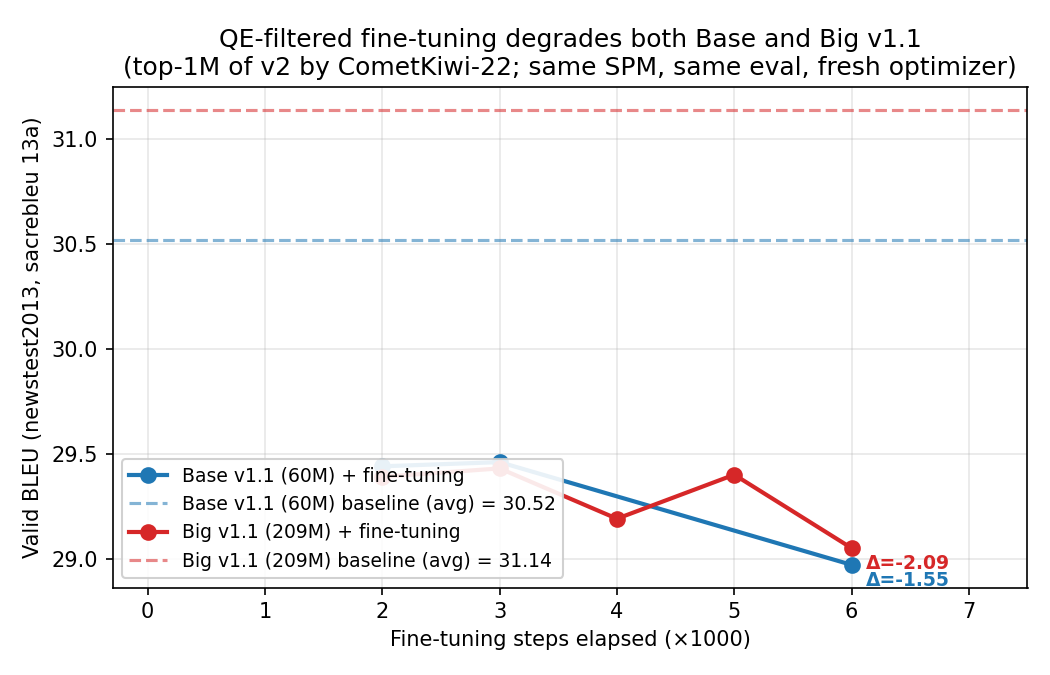
\includegraphics[width=\columnwidth]{figures/sft_curves.png}
\caption{Validation BLEU (newstest2013, sacrebleu 13a, beam=5, length-penalty=1.0) during QE-filtered fine-tuning. Solid lines are single-checkpoint evaluations during fine-tuning; dashed lines are pretraining baselines (5-checkpoint averaged). Both Base v1.1 (blue) and Big v1.1 (red) drop monotonically below their baselines. The first fine-tuning eval (step $+2$K) loses approximately 1 BLEU; subsequent steps drift further. Big drops more than Base.}
\label{fig:sft_curves}
\end{figure}

Training loss on the FT set converges smoothly from ${\sim}3.5$ (the pretraining floor on v1) to 1.94 (Base FT floor); the loss curve shows no sign of optimization failure. Sample translations during FT remain fluent and grammatically correct; accented French characters (\textit{Israël}, etc.) are preserved (no \texttt{<unk>}) thanks to the v1.1 SPM. \textbf{The drop is not a translation-quality collapse --- it is a distribution shift.}

Two observations from these numbers anticipate the analysis:
\begin{enumerate}
\item Big loses more than Base on both splits ($-0.79$ test, $-0.54$ valid). The architectural property that makes Big a better learner of clean in-distribution signal also makes it more pliable to whatever distribution it is fine-tuned on.
\item The FT-degraded models land near their v2-pretrained counterparts: Base$+$FT test 33.77 $\approx$ Base v2 test 33.90; Big$+$FT test 33.54 $>$ Big v2 test 33.03. Two genuinely different failure modes --- pretraining on noise (\S\ref{sec:enfr_v2}) and FT under a domain-mismatched filter (\S\ref{sec:sft}) --- converge to the same 33--34 BLEU band. We argue in \S\ref{sec:why_failures_differ} that this is not coincidence.
\end{enumerate}

\subsection{Why the filter selected what it did}
CometKiwi-22 is reference-free: it scores translation quality in absolute terms. The top-5 highest-scored pairs after deduplication are dominated by UN, intergovernmental, and legislative parallel data --- long, formal, syntactically rigid sentences with statistical content, professionally translated (Table~\ref{tab:top5_samples}).

\begin{table*}[t]
\centering
\small
\begin{tabular}{p{0.5cm} p{6.5cm} p{6.5cm} p{2cm}}
\toprule
\# & Source (en) & Translation (fr) & Domain \\
\midrule
1 & \emph{It is estimated that there are 500--650 million persons with disabilities in the world, approximately 10\% of the world population, 150 million of whom are children.} & \emph{On estime qu'il y a entre 500 et 650 millions de personnes handicapées dans le monde, soit environ 10\% de la population mondiale; 150 millions d'entre elles sont des enfants.} & UN report \\
\addlinespace
2 & \emph{The estimated number of people living with HIV in Eastern Europe and Central Asia rose to 1.5 million in 2007; almost 90\% of those infected live in either the Russian Federation (69\%) or Ukraine (29\%).} & \emph{On estime que le nombre de personnes vivant avec le VIH en Europe orientale et en Asie centrale a atteint 1,5 million en 2007; près de 90\% des personnes infectées vivent soit en Fédération de Russie (69\%) soit en Ukraine (29\%).} & UNAIDS \\
\addlinespace
3 & \emph{Since 2005--2006, the Government has reduced the federal debt by \$37 billion.} & \emph{Depuis 2005--2006, le gouvernement a réduit la dette fédérale de 37 milliards de dollars.} & Gov. \\
\addlinespace
4 & \emph{During 2006, the population of Finland increased by 4 per cent (21,375 persons).} & \emph{En 2006, la population finlandaise a augmenté de 4\,\% (21\,375 personnes).} & Stat. \\
\bottomrule
\end{tabular}
\caption{Top-4 highest-scoring v2 pairs by CometKiwi-22 (after deduplication; score band 0.8959--0.9145). The top scorers are professionally-translated UN/intergovernmental/legislative documents; WMT14 newstest is news domain.}
\label{tab:top5_samples}
\end{table*}

This is unsurprising: such corpora exhibit the alignment, completeness, and syntactic correspondence that QE is trained to reward. WMT14 newstest, in contrast, is news-domain --- looser register, shorter sentences, conversational interjections, named-entity-rich, with occasional ungrammaticality from quoted speech.

We thus have two distributions: an FT distribution (high-quality, formal, document-style) and an eval distribution (high-quality, informal, news-style). FT pulls the model's output distribution toward the former. On the FT distribution itself the model improves; on the eval distribution it gets worse, because every FT step trades news-style fit for formal-style fit.

\textbf{The model is not deteriorating in absolute quality.} It is being relocated in distribution space, and that relocation moves it away from the eval distribution.

\subsection{Implication: ``data quality'' decomposes}
This negative result refines the central claim of the paper:
\begin{quote}
Capacity return is determined by data quality. \emph{(\S\ref{sec:enfr_v1}--\S\ref{sec:ende})}
\end{quote}
\S\ref{sec:sft} forces a decomposition of ``quality'':
\begin{quote}
\textbf{Data quality = (translation correctness) x (alignment to target distribution).}
Both dimensions matter, and they are independent. Reference-free QE metrics measure the first; they do not measure the second.
\end{quote}

A naive top-K-by-QE filter optimizes only the first axis, and on a heterogeneous corpus (which v2 is --- news, web, UN, Europarl, all mixed) this can move the data far from the target eval distribution. The cleaner the QE filter, the more pronounced the domain skew, because high-quality parallel data is disproportionately UN/legislative.

This generalizes: any post-training step that filters on absolute quality without conditioning on the eval distribution risks moving the model away from where it should land. The fix is not ``better QE'' --- CometKiwi-22 is doing exactly what it should --- but \emph{domain-conditional filtering}: filter by QE within news-domain candidates, sample uniformly across domains within a QE band, or apply a domain classifier as a hard pre-filter.

\subsection{Why the v2-pretraining failure and the FT failure are different mechanisms}
\label{sec:why_failures_differ}

It is worth distinguishing the two failure modes the paper has now exhibited (Table~\ref{tab:two_failures}).

\begin{table}[t]
\centering
\small
\begin{tabular}{p{2.4cm} p{2.4cm} p{2.4cm}}
\toprule
& v2 pretraining (\S\ref{sec:enfr_v2}) & FT (\S\ref{sec:sft}) \\
\midrule
Data & all 30M v2 (noisy) & top-1M (clean) \\
Mechanism & wrong supervision & wrong distribution \\
Big$-$Base $\Delta$ & $-0.87$ & $-0.79$ (test) \\
Lesson & filter for noise & match for distribution \\
\bottomrule
\end{tabular}
\caption{Two failure modes producing $\sim$~33--34 test BLEU on newstest2014. Both amplify with capacity at comparable magnitude. The Big$-$Base $\Delta$ row reports test-BLEU differences (sacrebleu 13a, beam=5, lp=1.0; pretraining figures averaged, fine-tuning figures single ckpt as in Table~\ref{tab:sft_results}).}
\label{tab:two_failures}
\end{table}

These failures are independent axes. CometKiwi-based quality filtering \emph{does} address the v2 noise problem --- inspection of low-scored v2 pairs confirms that genuine noise concentrates at the bottom of the distribution --- but it does not address the distribution-alignment problem, because high-quality translations exist in many domains and our top-K selector does not condition on domain.

\textbf{Both failure modes appear to amplify with capacity.} Big v2 falls below Base v2 by 0.87 (noise amplification); Big FT falls below Base FT by $0.54$--$0.79$ (distribution-shift amplification). A reading consistent with current evidence: the architectural property --- more parameters, more representational capacity --- that makes Big a better learner of correct supervision on clean in-distribution data also makes it a more efficient absorber of incorrect supervision and a more pliable conformer to whatever distribution it is fine-tuned on. Under this reading, capacity acts as a force multiplier whose sign depends on the data, not on the model. With $n{=}1$ seed per cell, we frame this as a hypothesis supported by the four data points we report, not an established mechanism.

\subsection{Limitations}
\begin{itemize}
\item \textbf{Single seed.} Variance in FT outcomes is small relative to the $-1.55$ to $-2.33$ effects, but a 3-seed mean would tighten the bound.
\item \textbf{No low-LR FT.} A peak LR $\leq 5\text{e--}5$ might find a ``shallow FT'' point that improves UN-style without hurting newstest. We expect the effect to scale with effective FT distance from baseline; very-low-LR FT is slow to test, and the paper's claim does not require it.
\item \textbf{No domain-conditional filtering.} Building a news-conditioned top-K filter is a nontrivial sub-project (domain classifier $+$ quality scorer $+$ joint sampling). We flag it as the natural fix and leave it to future work.
\end{itemize}

\subsection{Headline}
Quality-filtered FT, on its own, does not improve newstest BLEU when ``quality'' is measured by reference-free QE on a multi-domain corpus. It costs 1.5--2.3 BLEU on Base / Big v1.1. The cause is not filter failure --- the filter selected genuinely high-quality pairs --- but that absolute translation quality and alignment to the eval distribution are independent axes of ``quality'', and only the first was optimized. The negative result tightens the paper's prescription:

\begin{quote}
\textbf{Filter first (for noise), match the evaluation distribution second (for register/domain), and only then scale capacity.} Skipping the second step undoes the capacity returns from the first.
\end{quote}
